\documentclass[UKenglish]{libraries/svproc}
%\documentclass[UKenglish]{svproc}

% Localisation
\usepackage{babel}
\usepackage{csquotes}

% Bibliography
\usepackage[alldates=long, sorting=none]{biblatex}
\addbibresource{rubik_f.bib}

% Misc.
\usepackage{amsmath}
\usepackage[export]{adjustbox}
\usepackage{wrapfig}
\usepackage{subcaption}
\usepackage{float}
\usepackage{textcomp}

% Tables
\usepackage{ctable}
\setupctable{botcap}

% URLs
\usepackage{url}
\urlstyle{rm}

% Hyperlinks (load last)
\usepackage[hidelinks]{hyperref}

%%% Project Information

\title{Rubik's Cube: Artificially Intelligent Solvers}
\subtitle{CS7IS2 Project (2020/2021)}
\author{
  William O'Sullivan   \and
  Basil Contovounesios \and
  Talha Ijaz           \and
  Fionnt\'an \'O Suibhne}
\institute{\email{
    wosulliv@tcd.ie,
    contovob@tcd.ie,
    ijazm@tcd.ie,
    suibhnef@tcd.ie}}
\authorrunning{O'Sullivan, Contovounesios, Ijaz, \'O Suibhne}

\begin{document}

\mainmatter
\maketitle              % typeset the title of the contribution

\begin{abstract}

An investigation into solving Rubik's Cubes by applying the following AI strategies was performed:
\begin{itemize}
    \item Genetic Algorithms (GA)
    \item Deep Reinforcement Learning + A$^{\ast}$ Search (DRL + A$^{\ast}$)
    \item Simulated Annealing (SA)
\end{itemize}
These approaches were used in order to determine solutions to a $2\times 2\times 2$ ($n=2$) ``Pocket Cube'' and a classic $3\times 3\times 3$ ($n=3$) Rubik's Cube.

The techniques broadly met with success, with every technique achieving a solution for a randomised cube. Times taken to solve each configuration varied between each instance, as did the number of turns required by each method to reach a solution. The DRL + A$^{\ast}$ method required the most up-front time due to its training component, but it resulted in consistent fast and efficient solutions. The novel GA solved every Pocket Cube and 27\% of Rubik's Cubes. Finally, SA resulted in very quick solutions for the Pocket Cube, and completed every Rubik's Cube, but required many turns to do so. 

\keywords{genetic algorithms, deep reinforcement learning, simulated annealing}

\end{abstract}

\section{Introduction}
%WRITING HERE
\subsection{Motivation}
1974 saw many historical events, including the election of the first female President of Argentina and ABBA's victory at the Eurovision with their iconic hit ``Waterloo''. 1974 also bore witness to the invention of the Rubik's Cube, a puzzle which has been in the minds of both pure mathematicians and computer scientists alike for decades. Whilst the puzzle has now been bested (even giving rise to the phenonmenon of Speedcubing!) it still serves as region of interest in fields where there is more concern for the method of solution.\\

Puzzles have long been a useful tool for examining the utility of artificial intelligence. Puzzles provide us with what would be considered an intellectual challenge, and creating agents that can produce solutions to puzzles can give us greater insight into both the limitations of such intelligences, as well as their strengths highlighting key areas where AI may find further use.

In the specific case of this investigation, we examine different agents for the problem of solving a Rubik's Cube, or indeed its smaller cousin the $2\times 2\times 2$ Pocket Cube, which will generally be described in the same way as it is simply a variant with a smaller state space. This particular puzzle sits at a cross-roads in terms of analysis. The Rubik's Cube is by no means a trivial pathfinding algorithm owing to the importance of move order but neither is it a puzzle without a known solution. That said, the Rubik's Cube itself only represents one member of a family of similar puzzles, for example higher dimensional $2\times 2\times 2\times 2$ objects, or longer sided $4\times 4\times 4$ cubes. A number of researchers have spent time investigating different methods of solving the cube via these intelligent agents only for some to determine that their approach does not suit the Rubik's Cube, whilst others meet with successful solutions.

At the outset, it was not expected that all of the approaches would yield perfect solutions to the Rubik's Cube. The heart of the investigation is built around understanding the methods and their applications in order to solve problems of this type, and this report will endeavour to share those findings accordingly.

\emph{NOTE: INCLUDE ONE\_DRIVE LINK}

\section{Related Work}
In keeping with the directive that the focus of the investigation should be on recent solutions of this field of problem, one group have been quite prolific in their publications on Rubik's Cube solvers in particular. The work of Stephen McAleer, Forest Agostinelli, Alexander Shmakov and Pierre Baldi~\cite{mcaleer2018solving, mcaleer2019solving, agostinelli2019solving} formed a consistent basis of understanding for the Rubik's Cube problem as a whole, whilst also drawing attention to the use of Deep Reinforcement Learning centred around their DeepCube solver. It was possible for the researchers to use the policies determined by DRL with different search approaches, including Monte Carlo Tree Search (MCTS) and A$^{\ast}$ Search.

Beyond the use of DRL, however, lay two other approaches which draw influence from biology and physics, in Genetic Algorithms and Simulated Annealing respectively.

Genetic Algorithms are a way of generating increasingly close approximations to a solution, to the point where a solution itself is achieved. The work of El-Sourani et al.~\cite{10.1007/978-3-642-12239-2_9} utilised GA to solve a Rubik's Cube by incorporating the analytical solution to a Rubik's Cube based on the original work by Thistlethwaite~\cite{Thistlethwaite}. Whilst this technique resulted in solutions for any given cube configuration, Smith et al.~\cite{10.1145/2908812.2908887} attempted to build on this by determining policies with their GA rather than determining configuration-unique solutions, ultimately meeting with a great degree of success.

Simulated Annealing is a kind of random search method not unlike the aforementioned MCTS, however it possesses an additional strength in that it is also an iterative improvement algorithm. This means that the SA approach is able to escape local extrema, whilst consistently improving performance. SA has seen use in solving Sudoku puzzles, as in the work of Lewis~\cite{SAarticle}, and indeed SA could be applied to solving Rubik's Cubes by tweaking how the cost function is determined.

Between the applications of DRL + MCTS, DRL + A$^{\ast}$, GA for values, GA for policies and SA, a decision was made to investigate the properties of DRL + A$^{\ast}$, GA for values, and SA.

DRL + A$^{\ast}$ was selected as an investigation into the most modern approach to solving Rubik's Cubes. GA for values would allow for investigation of the differences between performance on $n=2$ and $n=3$ cubes without the added complexity of trying to determine policies for the different sized cubes. Finally, SA was selected in order to examine the effects of stochastic solvers in Rubik's Cubes, which had been scarcely investigated.

Overall, the proposed techniques comprise a decent and broad collection, and draw on a diverse set of approaches to solve one popular problem.

It should be noted that an implementation~\cite{Shoukat2019} based the work of Korf~\cite{KORF198597} was used as a baseline for comparison in terms of runtime. It is important to note that this algorithm does rely on human (domain) knowledge however, and so acts not as a baseline to beat necessarily, but a good comparison between the agents which do not have human knowledge, and those that do.


\section{Problem Definition and Algorithm}
The Rubik's Cube for both $n=2$ and $n=3$ is a sparse state space problem, meaning that only one solution exists in an otherwise very large state space. This presents unique challenges to finding suitable techniques for devising solutions to the cubes.

\subsection{Deep Reinforcement Learning + A$^{\ast}$ Search}
Reinforcement Learning (RL) involves exploring state spaces in order to determine optimal policies for maximising rewards. In the case of a Rubik's Cube, the state space is incredibly sparse with $\sim 10^{19}$ possible states and only one solution. As such, classical RL is insufficient to solve a Rubik's Cube, leading to the requirement of DRL. DRL utilises Deep Learning to more efficiently operate over a large state space by eliminating the need to store it directly. Instead, models are trained to compute effective outputs from unstructured inputs by iteratively approximating a function of the domain.
Unfortunately, even with these advanced techniques the Rubik's Cube proved unsuitable for solving with DRL alone. The sparse nature of the problem means that the learning element can often fail to propagate rewards from the goal state. To alleviate this problem, the way in which the DRL training occurs is reversed; rather than starting with a randomised cube and trying to solve from there, a solved cube is randomised with the agent knowing how the random state was reached. This is called Autodidactic Iteration, and ensures that every training instance can result in a solution. It is in this way that training samples for the DNN can be selected to yield a useful basis for training a `cost-to-go' function $J$ that estimates the number of moves of a given state $s$ from the goal state. Training the DNN involves minimising the MSE between the current $J(s)$ and its update $J'(s)=\min_aJ(A(s,a))$, where $A(s,a)$ is the state resulting from taking action $a$ in $s$, in a process named Deep Approximate Value Iteration~\cite{agostinelli2019solving}.
The trained function can then be used to inform a search strategy for solving Rubik's Cubes. Greedy Best-First Search was found to perform badly with more scrambled cubes, so a weighted A$^\ast$ Search with the following cost function $f$ is used instead:
\begin{align*}
  f(x)&=\lambda g(x)+h(x),\qquad\lambda\in [0,1] \\
  h(x)&=\begin{cases}
    0    & \text{if $x$ is the goal node} \\
    J(x) & \text{otherwise}
  \end{cases}
\end{align*}
Controlling the weighting factor $\lambda$ on the current path cost function $g$ can afford better runtime characteristics at the expense of optimality. To further offset the DNN evaluation overhead, the frontier is expanded in parallel batches, giving rise to Batch Weighted A$^\ast$ Search (BWAS).  This investigation examined the effects of varying $\lambda$ on runtime efficiency and solution optimality, with empirical results presented in Figure~\ref{fig:fig3}. 

\subsection{Genetic Algorithms}

\begin{figure}[!h]
\begin{small}
\centering
\linespread{1.0}
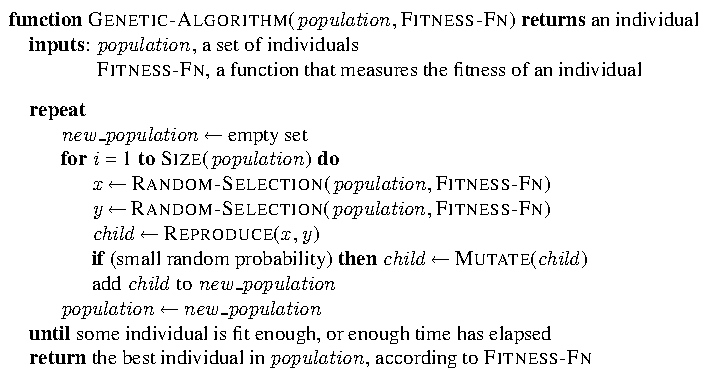
\includegraphics[width=0.9\linewidth]{images/genetic-algorithm}
\caption{Genetic Algorithms utilise reproduction, whereby a parent passes its characteristics onto its child. Over several generations an individual that better satisfies the fitness criteria emerges~\cite{10.5555/1671238}.}
\label{fig:fig0}
\end{small}
\end{figure}

GA define populations as a set of approximate solutions, with each individual representing one such attempt. Certain individuals are better suited to meeting fitness criteria (i.e. how well a solution conforms to the required behaviour) and so upon the passage of a generation, individuals with better fitness have a higher probability to reproduce, creating a new individual with characteristics from two previous approximations. However, reproduction is not the only way in which the population evolves. Concepts of mutation and elitism allow for the propagation of individuals with desirable traits as well. Overall, the passage from one generation to the next is composed of 60\% offspring, 30\% by mutation and 10\% by elitism. Offspring come about based on the previous notion of reproduction, whilst mutants are the result of lone individuals experiencing a number of small move alterations, and elitism allows for the propagation of the portion of the population that was judged to be most fit. The elites are selected from the best population that did not produce offspring, as to give them another chance to reproduce. To maintain diversity, if an individual was allowed to breed or mutate, it could not be carried along via elitism.

The idea is that these new individuals will possess a combination of attributes that allow them to satisfy the fitness function even better, in turn increasing the chance of their characteristics being passed along. In this manner that mimics natural selection, over a number of generations it becomes possible to arrive at a population that contains individuals which satisfy the fitness criteria perfectly, at which point a solution has been reached.

In this investigation, GA were used to solve a Rubik's Cube without human knowledge. The analytical solution modified the fitness criteria at different stages, in accordance with the Thistlethwaite methods, such that the direction of evolution was modified to become increasingly adept at solving the Rubik's Cube in a low number of steps.  This particular implementation however did not alter the cost function at any point, and so the GA could only act to minimise the following cost function:
\begin{align*}
  \text{All elements of a row} &
  \begin{cases}
    +0 & \text{all colours uniform} \\
    +1 & \text{all colours not uniform}
  \end{cases} \\
  \text{All elements of a column} &
  \begin{cases}
    +0 & \text{all colours uniform} \\
    +1 & \text{all colours not uniform}
  \end{cases} \\
  \text{All elements of a face} &
  \begin{cases}
    +0 & \text{all colours uniform} \\
    +1 & \text{all colours not uniform}
  \end{cases}
\end{align*}
This cost function was used to select for elitism and breeding, as well as for meeting the termination criterion - a cost 0 cube arose in the event of a solution. The algorithm would also terminate in the event that an iteration threshold was exceeded, indicating that the cube had become stuck in a degenerate state and failed to solve.

\subsection{Simulated Annealing}

\begin{figure}[!h]
\begin{small}
\centering
\linespread{1.0}
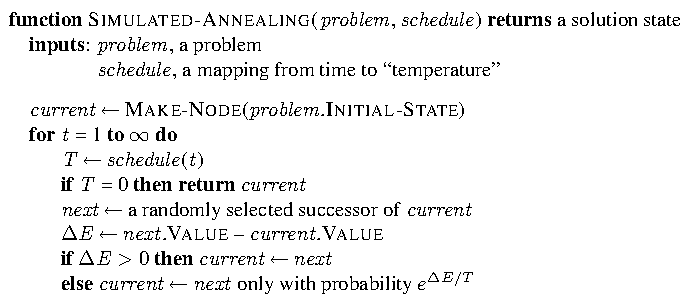
\includegraphics[width=0.9\linewidth]{images/simulated-annealing}
\caption{By slowly approaching a solution state using a controlled stochastic method, Simulated Annealing results in a solved system~\cite{10.5555/1671238}.}
\label{fig:fig1}
\end{small}
\end{figure}

SA begins as a process with an initial random state with a corresponding initial ``temperature''. This temperature affects the probability of accepting unfavourable moves that diminish the overall fitness of the current state. Whilst this may sound counter-productive, it is very important for preventing the Rubik's Cube from becoming stuck in a degenerate state, whereby it is unable to access moves that would diminish the cost function even further than the present state. This is a critical aspect of solving the puzzle on account of the fact that moves in Rubik's Cubes are non-commutative, that is to say, a move left followed by a move up is not identical to a move up followed by a move left. After a number of moves have occurred, the temperature begins to decrease, reducing the probabilities of accepting less favourable moves. This process continues until the system ``cools'' and either a solution has been reached, or the system is then ``reheated'' in a bid to shuffle around moves and solve the cube outright. Having specified parameters such as the initial temperature and cooling rate of the system, it was possible to investigate the effects of modifying these parameters to see whether a solution would successfully converge or not.

%This section formalises the problem you are addressing and the models used to solve it. This section should provide a technical discussion of the chosen/implemented algorithms. A pseudocode description of the algorithm(s) can also be beneficial to a clear explanation. It is also possible to provide one example that clarifies the way an algorithm works. It is important to highlight in this section the possible parameters involved in the model and their impact, as well as all the implementation choices that can impact the algorithm.


\section{Experimental Results}

\subsection{Methodology}
The solutions to both the Pocket Cube ($n=2$) and Rubik's Cube ($n=3$) were evaluated using two general criteria where they could be applied, counting the number of moves that a method took to reach a solution, and measuring the time taken for an individual solution to a newly randomised cube.

Whilst the DRL + A$^{\ast}$ solution for the $n=2$ and $n=3$ cubes was built upon the existing DeepCube environment, the GA and SA approaches required a custom test environment in which a cube could be evaluated in terms of cost and solution.

\subsubsection{Shared Basis for GA and SA}
Before any algorithms could be applied a test environment had to be constructed. A \verb|RubiksCube| object was constructed containing several features:
\begin{itemize}
    \item A method for determining the current `cost' of the cube. A solved Rubik's Cube would have a cost of 0, with displacement from a solved state resulting in an increased cost which scaled with $n$, the dimension of the cube. The specific way in which cost was determined was then unique for each technique.
    \item A method to generate a random move, and from that a method to randomise the cube itself. This would allow the cube to initialise into a state following 30 to 40 randomisation operations.
    \item A method to apply either the random moves or a set of moves specified by the agent. Moves would be entered as a combination of a row/column specifier and a direction declaration.
\end{itemize}

\begin{figure}[!h]
\begin{small}
\centering
\linespread{1.0}
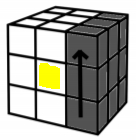
\includegraphics[width=0.2\linewidth]{images/move_3u.png}
\caption{Taking the nearer (highlighted) face as the frame of reference, this particular transformation would be described as a $[2,u]$ move. Using index notation, the third column of the face is rotated upwards by 90\textdegree~\cite{proj_l.hoang}.}
\label{fig:fig2}
\end{small}
\end{figure}

This cube could be manipulated, as in Figure~\ref{fig:fig2} by an agent in order to reach a solution after a successful set of moves had been made.

\subsection{Results}

Table~\ref{tab:res} presents the mean runtime and the mean number of moves for solving both the Pocket Cube and Rubik's Cube, over what were considered idealised parameters.

\ctable[
  pos = h!,
  caption = {Mean empirical metrics across cube sizes},
  label = tab:res
]{@{\extracolsep{1em}}ll*{4}{r}}{}{ \FL
  Size & Metric & DRL + A$^\ast$ & GA & SA & Baseline       \ML
  $n=2$ & Runtime (s) &            3.2 &  7 &  2.9 &       10 \NN
        & \# of Moves &            10 &  29 &  1270 &       17 \ML
  $n=3$ & Runtime (s) &           13.6 &  255 &  204 &       15 \NN
        & \# of Moves &           22 &  350 &  43623 &       32 \LL
}

%ROUNDING MOVE COUNT from 9.8->10 and 22.1->22 for DLR+A*
% NOTE: COULD USE KORF AS A BASELINE

\subsubsection{DRL + A$^{\ast}$}

\begin{figure}[!h]
\begin{small}
\centering
\linespread{1.0}
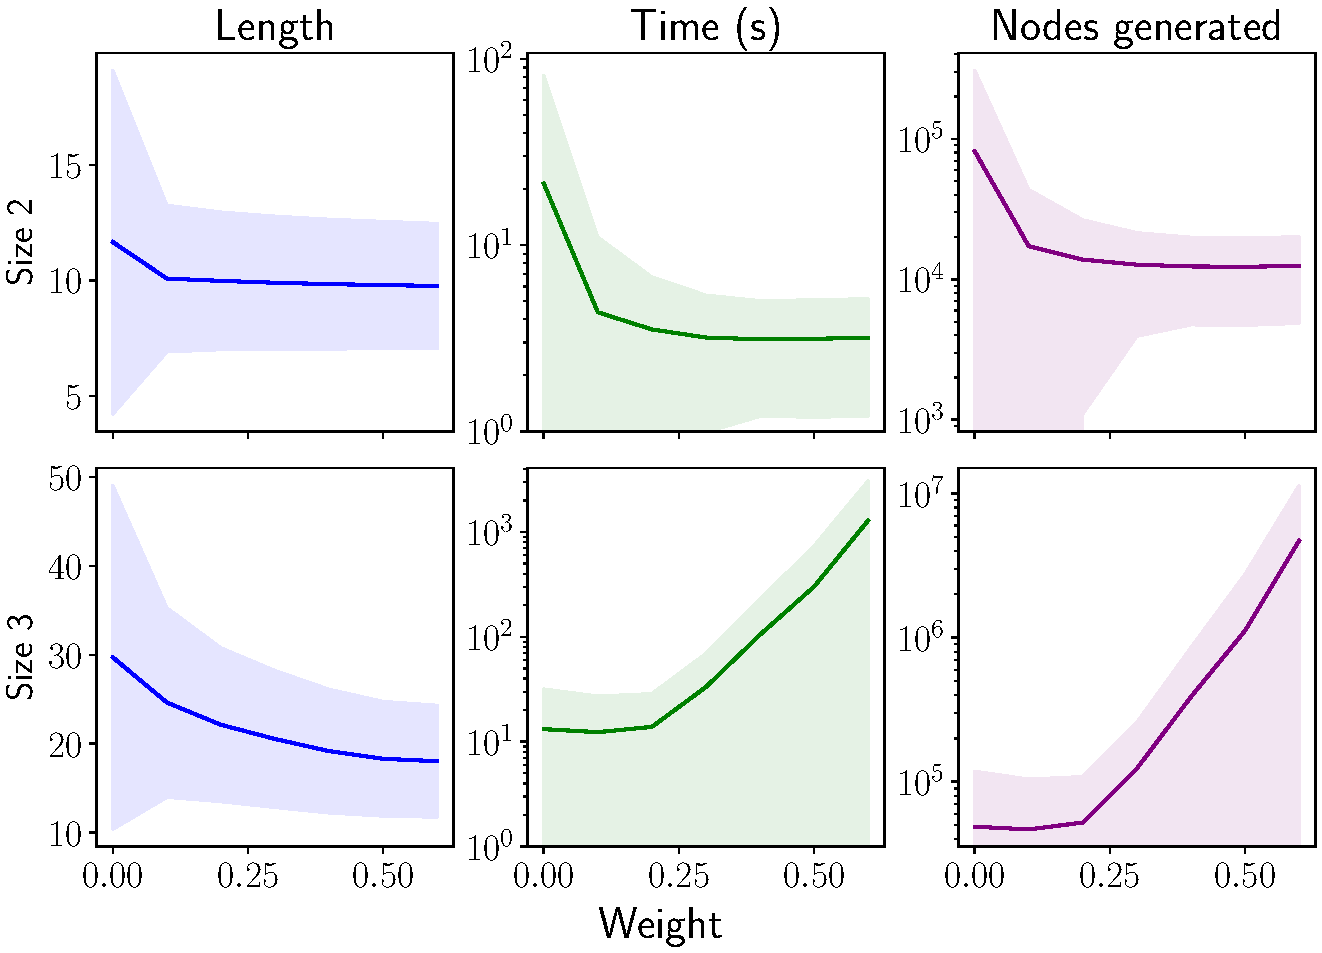
\includegraphics[width=0.8\linewidth]{images/bwas}
\caption{Mean BWAS solutions ($\pm\sigma$) for 100 runs on cubes up to 100 random moves away from the goal state, with a batch size of 100, on 16 AMD EPYC 2nd Gen. CPUs. The length of a solution is also known as the number of moves required to reach a solved state.}
\label{fig:fig3}
\end{small}
\end{figure}

Figure~\ref{fig:fig3} displays how the A$^{\ast}$ Search varied with weighting. Surprisingly, the difference in behaviour between the $n=2$ and $n=3$ can be seen in how the weighting drives performance. In the $n=2$ case, increasing the weighting reduces the move count as in its $n=3$ counterpart. However, it has the additional effect of driving down the runtime (which proportionally scales with the nodes expanded) as well, which directly contradicts the behaviour of the $n=3$ model. This peculiar behaviour arises due to the Pocket Cube possessing only a little over 3.5 million unique states - practically insignificant when compared with the more than 4 quintillion unique states of the Rubik's Cube. The number of nodes that need to be generated to reach a solution is diminished accordingly. \par The behaviour we observe in the Rubik's Cube is more typical of our expectations - increasing the weighting drives the agent to find more efficient solutions, but at the cost of increased runtime.

\subsubsection{GA}
The values in Table~\ref{tab:res} were obtained for a population of 150 for a move limit of 450.
In the $n=2$ case, the GA regularly solved the cube faster than the baseline, even though it did require more moves to do so. In the $n=3$ case, the genetic algorithms tended to become stuck in a local cost minima very close to the final solution, meaning that 73\% of randomised cubes went unsolved. More than 80\% of the failed attempts yielded a best cost below 20 and more than 60\% of the failed attempts had a best cost below or equal to 12. A cost of 12 just meant one misplaced corner (8 out of 9 tiles on each face match). 
While the Rubik's Cubes were not solved, proximity to the solution would enable the use of domain knowledge complete the mostly solved cube. The domain knowledge could be implemented as heuristics, hard coded as rules. For example a certain sequence could have been employed upon reaching a cost of 12 in order to finish out the cube. That said, even in the absence of domain knowledge the GA was still capable of determining its own solutions 27\% of the time.

\subsubsection{SA}
The values in Table~\ref{tab:res} were obtained for a starting temperature of 35, a cooling rate of 0.99, and a final temperature of 0.01. This starting temperature enabled the selection condition to accept a random move around 80\% of the time, until random moves were very seldom selected around the final temperature.
SA was characterised primarily by its very long move count, for both $n=2$ and $n=3$, but such behaviour was to be expected - the stochastic method did not learn nor did it inherit beneficial characteristics from prior moves. Each move was only concerned with the state as it was. Additionally, by virtue of accepting random moves the move count was expected to bloat regardless. The surprising result however was in how quickly the SA was able to act - at 2.9 seconds the SA beat not only the baseline, but also the DRL + A$^{\ast}$ and GA method for the $n=2$ case, despite having over almost 40 times the number of moves. The SA continued to beat the the GA in terms of runtime, for the $n=3$ case despite again requiring an enormous number of moves to solve.

\subsubsection{Baseline}
The baseline used was an Iterative-Depth A$^{\ast}$ Search, which availed of domain knowledge. This was an august technique for solving Rubik's Cubes in less than 20 moves with a readily available implementation~\cite{Shoukat2019}. 

\subsection{Discussion}
It should be noted that the common metric used by the models, that is runtime and number of moves, immediately runs into a dilemma---should the training time for the DRL + A$^{\ast}$ model included when measuring solution time?  One could argue either way, but it is important to highlight that whilst the DRL + A$^{\ast}$ ran fastest, there was certainly a significant degree of overhead to its use. It was only by the virtue of using the DRL to create a lookup table that DRL + A$^{\ast}$ was able to compete for the $n=3$ cube whereas the other models had to develop the solution from zero domain knowledge each time.

Beyond that lay the parameters unique to each model, be it the architecture and hyperparameters of the DNN, the A$^{\ast}$ batch size and weightings, the rate of mutation in the GA or the cooling rates in the SA. Modifying these values has well understood implications when the problems are treated in tandem---it is possible to see that in the case of GA and SA high mutation rates and high starting temperatures increase the time taken to arrive at a solution state, and yet such an analogous relationship does not exist for the DRL + A$^{\ast}$. However, one could (inelegantly) compare the number of generations in a GA with the number of layers in the DNN used in the training process, arguing that many inputs are taken to ultimately return a unique item of use. According to present understanding, there is no such trait that can be described as truly common between the three methods employed in this investigation; where one analogy holds for two techniques, it either fails to capture the third outright or else makes the vaguest approximation to what is actually going on within the model.

Whilst behaviour between the differing models was very difficult to compare for the $n=3$ scenario, it cannot be denied that the performance was very consistent; indeed, one can readily see between the three models that there is an interesting balance between the time taken and the number of moves to solve. The SA required a tremendous number of moves to solve, but ran the fastest, whereas the DRL + A$^{\ast}$ method very effectively minimised the number of turns required. GA seemed to position itself as an approach that took time to determine a fairly optimal configuration whilst taking a modest amount of time to run.

Completeness of solutions is another criteria on which the models can be judged. Whilst the GA did solve every $n=2$ cube, $n=3$ cubes required longer sequences of moves, resulting in difficulty in solution. When many individuals in such a population had identical fitness, it became difficult for more favourable traits to propagate effectively. DRL + A$^{\ast}$ and SA did not encounter this dependency issue, with the former guaranteed solution states by ADI, and the latter continually marching on until a solution was located. It can be conjectured that were the GA not to be limited by the number of iterations, it too would have achieved the same completeness after the degeneracy had either mutated out, or a new offspring had just the right parents in a far off generation.

\section{Conclusions}
The investigation of artificially intelligent Rubik's Cube solvers without domain knowledge was a success - all three approaches Deep Reinforcement Learning + A$^{\ast}$ Search, Genetic Algorithms and Simulated Annealing were able to solve Rubik's Cubes without any additional shortcuts or heuristics being provided. 

Ultimately, the GA and SA could see improvement in future versions by inclusion of such heuristics to resolve the issue of being trapped in degenerate states. That said, the GA and SA approaches implemented in this investigation was the first of their kind - GA had previously been used with domain knowledge, and SA had been used to solve similar sparse state space problems, but these unique implementations demonstrate that techniques beyond DRL + A$^{\ast}$ search can solve the timeless Rubik's Cube without the help of humans.

\clearpage
\printbibliography
\end{document}